\chapter{Implementácia vybraných útokov}

\label{kap:implementacia} % id kapitoly pre prikaz ref

V tejto kapitole podrobne popíšeme vybrané útoky na konkrétny hardvér, ktoré sa nám podarilo uskutočniť.

\section{Útok na firmvér zo súťaže CTF}
Ako prvé sme sa pokúsili zreprodukovať popísaný útok na firmvér, ktorý bol realizovaný v rámci súťaži CTF (Capture The Flag) \cite{vccOnTheCheap}. Firmvér po spustení periodicky posiela cez rozhranie USART (Universal Synchronous / Asynchronous Reciever and Transmit) správu \uv{Lock}. Po úspešnom útoku by mal poslať \uv{tajný flag}, ktorého obsah je cieľom tejto súťaže. Potrebný hardvér pre realizáciu tohoto útoku je nasledovný:
\begin{itemize}
    \item Arduino UNO R3 -- použili sme precízny klon, obsahuje vyberateľný čip ATMega328P v THT púzdre
    \item Arduino Nano -- taktiež precízny klon, použité na ovládania tranzistora ako zdroj indukovania chýb
    \item kontaktné nepájivé pole -- umožňuje jednoducho prepájať súčiastky bez potreby spájkovania
    \item bipolárny tranzistor NPN -- model 2N2222A v THT púzdre
    \item rezistory -- použili sme 2-krát 330$\Omega$, potrebný odpor sa môže líšiť v závislosti od použitého tranzistora
    \item prepojovacie kábliky typu M-M (Male to Male), niekoľko (približne 15) kusov rôznej dĺžky
\end{itemize}
Čo sa týka softvéru je potrebný ISP programátor, ktorý dokáže nahrať firmvér na mikrokontrolér ATMega328P a kompilátor jazyka C pre architektúru AVR. Použili sme integrované vývojové prostredie (IDE) Arduino IDE, ktoré poskytuje automatizovaný spôsob kompilovania a nahrávania firmvéru, podporujúce aj náš ATMega328P. Firmvér, na ktorý chceme útočiť bol poskytnutý priamo v skompilovanej forme a pre nahranie takéhoto kódu sme priamo použili open source projekt AVRDUDE, ktorý interne používa aj Arduino IDE.

\subsection{Postup útoku}
Postup je zhodný s popisom pôvodného útoku \cite{vccOnTheCheap}. Po prvé potrebujeme nahrať firmvér, na ktorý budeme útočiť na mikrokontrolér ATMega328P, ktorý je súčasťou dosky Arduino UNO. Doska obsahuje prevodník z USB na USART, čo zjednodušuje celý postup. Prevodník na doske pripojíme k počítaču a nahráme firmvér zo súťaže priamo pomocou softvéru AVRDUDE \cite{vccOnTheCheap}. Súbor \uv{fiesta.hex} so skompilovaným firmvérom, ktorý je potrebné nahrať sa nachádza v prílohe \ref{pri:softver}, prevzatý zo súťaže \cite{vccOnTheCheap}. 

Ďalšim krokom je hardvérové zapojenie. Mikrokontrolér ATMega328P vyberieme z dosky Arduino UNO, keďže doska obsahuje stabilizátor napätia, ktorý by útok znemožňoval. Následne zapojíme tranzistor, tak aby ho bolo možné spínať pomocou Arduino Nano -- emitor prepojíme so zemou na doske a bázu prepojíme s pinom, ktorý ovláda tranzistor (v našom prípade pin D2). Medzi doskami prepojíme piny zabezpečujúce sériovú komunikáciu USART smerom z UNO do Nano, aby bolo možné prečítať vypísaný \uv{flag}, pre tento účel je potrebné prepojiť aj zem medzi doskami. Vybratý čip ATMega328P v púzdre THT umiestnime na kontaktné pole a prepojíme (káblikmi) naspäť s pôvodnou doskou Arduino UNO nasledovné piny: 1, 2, 3, 7, 9, 10 a 20. Tieto zabezpečujú základné potreby pre fungovanie mikrokontroléra -- napájanie (zem týmto spôsobom neprepájame), externé hodiny (kryštál), sériová komunikácia. Piny 8 a 22 (zem), prepojíme s kolektorom tranzistora -- zopnutím tranzistora pomocou ovládacieho pinu Arduino Nano, takto vieme odpájať a pripájať ATMega328P so zemou. Podrobná schéma celého zapojenia sa nachádza na obrázku \ref{obr:schemeCTF}.

\begin{figure}
    \centerline{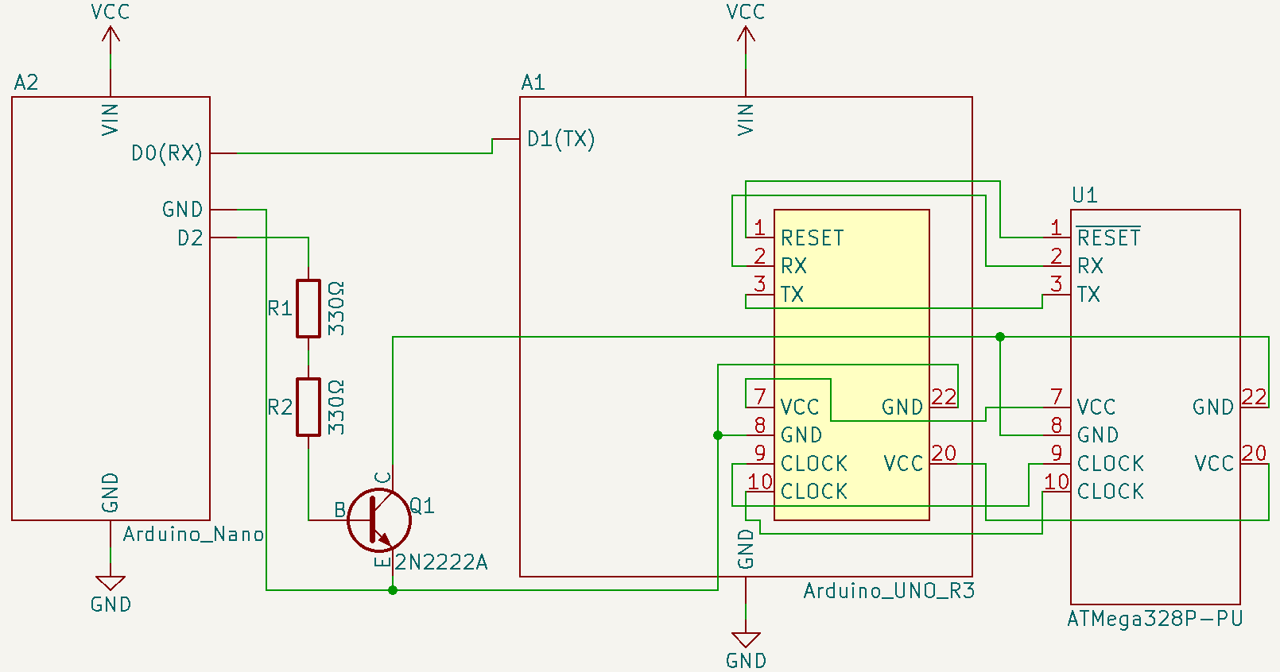
\includegraphics[width=1\textwidth]{images/schemeCTF.png}}
    \caption[Schéma zapojenia útoku na firmvér zo súťaže CTF]{Schéma zapojenia útoku na firmvér zo súťaže CTF \cite{vccOnTheCheap}. Žltý obdĺžnik znázorňuje nepájivé púzdro na doske Arduio UNO, z ktorého bol vybratý mikrokontrolér ATMega328P.}
    \label{obr:schemeCTF}
\end{figure}

Ďalej je potrebné naprogramovať Arduino Nano, aby pomocou ovládania tranzistora na krátko odpojilo napájanie ATMega328P od zeme a následne opäť pripojilo. Dĺžka časového intervalu, počas ktorého je tranzistor vypnutý, musí byť dostatočne dlhá, aby indukovala chybu na procesore, ale nie príliš dlhá, aby sa mikrokontrolér resetoval. Vyskúšali sme do Arduino Nano nahrať program použitý aj v pôvodnom útoku \cite{vccOnTheCheap}, ktorý bol implementovaný v prostredí Arduino IDE. Algoritmus vypne tranzistor a vykoná niekoľko prázdnych iterácií for-cyklu, po ktorom tranzistor opäť zapne. Následne sa pokúsi prečítať výstup zo sériového portu na ATMega328P. V prípade, že sa podarí prečítať \uv{flag}, útok bol úspešný. V prípade, že sa \uv{flag} nepodarí prečítať, zväčší počet iterácií for-cyklu a postup zopakuje \cite{vccOnTheCheap}. Ukážka časti kódu, ktorá ovláda tranzistor, je v algoritme \ref{alg:vccOnTheCheap}.

\begin{lstlisting}[float,language=C,caption={Ovládanie tranzistora, ktorý spína napájanie na ATMega328P. Prevzaté zo zdrojového kódu pôvodného útoku \cite{vccOnTheCheap}.},label=alg:vccOnTheCheap]
int waste = 0;
digitalWrite(powerPin, LOW);
for (int i = 0; i<glitchDelay; i++){ waste++; }                    
digitalWrite(powerPin, HIGH);
glitchDelay += 10;
\end{lstlisting}

\subsection{Výsledok, analýza a vylepšenie útoku}
Útok bol vyskúšaný na všetky štyri čipy ATMega328P. Na dvoch z nich sa útok úspešne podaril s rovnakým podobným výsledkom ako v pôvodnom popise \cite{vccOnTheCheap} a \uv{flag} sa podarilo prečítať už pri nulovom počte iterácií for-cyklu. Postačoval najkratší možný výpadok -- vypnutie a okamžité zapnutie tranzistora pomocou funkcií poskytnutých prostredím Arduino IDE. Na druhých dvoch exemplároch (z inej série výroby) útok nebol úspešný a aj pri tomto najkratšom možnom výpadku sa mikrokontrolér resetoval. Rozhodli sme sa preto napätie na mikrokontroléri počas útoku podrobne analyzovať pomocou osciloskopu. Pre tento účel sme sa rozhodli ATMega328P zapojiť na kontaktom nepájivom poli bez dosky Arduino UNO. Postup tohoto zapojenia sme popísali v kapitole \ref{kap:hardver}. Takéto zapojenie umožňuje meniť pasívne elektronické súčiastky v zapojení, čo poskytuje väčšiu flexibilitu vo voľbe parametrov týchto súčiastok pri analýze.

Pomocou osciloskopu sa podarilo podrobne určiť priebeh zmeny napätia na mikrokontroléri v čase s presnosťou na rádovo stovky nanosekúnd. Výsledkom bolo, že interval, počas ktorého nastalo podpätie bol príliš dlhý (približne 2 ms), čo pri útoku na 2 čipy zo štyroch spôsobilo reset mikrokontroléra. Doska Arduino Nano, ktorá ovládala tranzistor obsahuje tiež mikrokontrolér ATMega328P, s externým oscilátorom s frekvenciou 16 MHz. V kapitole \ref{kap:hardver} sme spomenuli ukážku nastavenia výstupnej logickej hodnoty na 1, resp. 0 pomocou jedinej inštrukcie SBI, resp. CBI. Obé tieto inštrukcie dokáže procesor vykonať počas dvoch taktov vďaka dvojfázovej pipeline (načítanie a vykonanie inštrukcie) \cite{atmegaData}. Pri frekvencii 16 MHz to znamená, že vypnutie a opätovné zapnutie tranzistora by teoreticky malo trvať 1/4 mikrosekundy. Ďalším zaujímavým pozorovaním je, že časový interval podpätia sa nepredlžoval so zväčšovaním počtu iterácií \uv{prázdneho} for-cyklu. Dôvodom môže byť optimalizácia kompilátora, ktorý sa oprávnene rozhodol zdanlivo \uv{zbytočný} for-cyklus odstrániť.

Rozhodli sme sa preto časti kódu, ktoré ovládajú tranzistor prepísať do jazyku asemblera s využitím C Inline Assembly, ktorý je podporovaný aj kompilátorom prostredia Arduino IDE. Volania funkcie \uv{digitalWrite} sme teda nahradili ekvivalentnou konštrukciou pomocou inštrukcií SBI a CBI. Následne sme útok zopakovali s takto upraveným programom nahratým na Arduino Nano. Výsledkom bolo, že podpätie na mikrokontroléri trvalo pripližne 1/2 mikrosekundy, čo je štyrikrát menej ako predtým. Rozdiel medzi teoretickým časom (1/4 ms), bol pravdepodobne spôsobený nedokonalosťou tranzistora a vplyvom ďalších fyzikálnych faktorov. Pri takto krátkom čase už nenastal reset žiadného z testovaných čipov, ale útok bol opäť neúspešný. Interval bol pravdepodobne príliš krátky a na žiadnom z čipov sa neprejavila chyba. Ďalej sme preto upravili kód napísaním vlastnej procedúry oneskorenia v asembleri (opäť s využitím C Inline Assembly). Procedúra pozostáva z inicializácie registra na kladnú hodnotu (osem-bitový parameter) a cyklu. V cykle postupne dekrementujeme tento register a následne vykonáme podmienený skok na začiatok cykla, pokiaľ výsledok dekrementu bol nenulový. Pseudokód procedúry v jazyku asemblera uvádzame v algoritme \ref{alg:asmDelay}. Takáto procedúra umožňuje parametrizovať oneskorenie s presnosťou na trojce taktov (cyklus procedúry trvá tri takty). Po tejto úprave sa útok úspešne podaril na všetkých štyroch testovaných čipov. Potrebné oneskorenia pre úspešný útok na každom z exemplárov sú zhrnuté v tabuľke \ref{tab:vccOnTheCheap2}. Väčšiu presnosť by bolo možné dosiahnúť vsnutím presného počtu inštrukcií NOP, medzi vypnutím a zapnutím tranzistora. Počet inštrukcií NOP, by však musel byť známy v čase kompilácie, čo by znemožnilo dynamicky upravovať dĺžku oneskorenia za behu.

\begin{lstlisting}[float,language=C,caption={Jednoduchá procedúra oneskorenia v asembleri. \{IN\} označuje vstupný parameter -- 8-bitová konštanta, alebo hodnota v registeri.},label=alg:asmDelay]
mov r24, {IN}   // 1 takt
loop:
    dec r24     // 1 takt
    brne loop   // 2 takty pri vykonani skoku, 1 inak
\end{lstlisting}

\begin{table}
    \caption[Porovnanie vylepšeného útoku zo súťaže CTF na rôznych čipoch ATMega328P.]{Porovnanie vylepšeného útoku zo súťaže CTF na rôznych čipoch ATMega328P. Čísla v tabuľke udávajú vstupný parameter (počet cyklov) procedúry oneskorenia. Na čipy zo série 2128BQY pôvodný útok nebol úspešný.}
    \label{tab:vccOnTheCheap2}
    \begin{center}
    \begin{tabular}{|c|c|c|c|}
        \hline 
        Séria čipu & Min (úspešný útok) & Max (úspešný útok) & Ideál (vždy úspešný útok) \\
        \hline
        2139E4A & 6 & 12 & 9--10 \\
        \hline
        2139E4A & 4 & 11 & 10 \\
        \hline
        2128BQY & 3 & 11 & 7 \\
        \hline
        2128BQY & 4 & 12 & 8--9 \\
        \hline
    \end{tabular}
    \end{center}
\end{table}